\subsection{Enrich Co-occurrence Matrix and Articles}
\label{sec:enrich}

%\KZ{
%{\bf OUTLINE}
%\begin{itemize}
%\item co-occurrence matrix
%\item Overview of EnrichMatrix function
%\item UpdateArticles, Scoring function
%\item UpdateMatrix
%\item How we handle general terms (boosting)
%\end{itemize}
%}

Co-occurrence among Wikipedia concepts provides
the knowledge for disambiguating terms in a given document.
The co-occurrence information of Wikipedia concepts is in theory
a $K \times K$ square matrix where $K$ is the total number of concepts in
Wikipedia. Each element in the matrix represents
the total co-occurrence frequency of the two concepts in
any Wikipedia articles.
Despite the large number of concepts that exist in Wikipedia, not every pair of
them co-occur, and therefore in practice, the matrix is very sparse and
manageable. Next, we present the algorithms that compute the co-occurrence
matrix, which involves two phases: {\em matrix initialization} and
{\em matrix enrichment}.
%And the end of the section, we
%discuss an important scoring function involved the enrichment process.

\subsubsection{Matrix Initialization}
In the initialization phase, we take as input the parsed Wikipedia articles
which include both linked terms and unlinked terms,
and calculate the co-occurrence frequency between the concepts of two linked
term and the appearance frequency of each concept
(i.e., the sum of all co-occurrence frequencies for that concept).
We argue that computing the co-occurrence within the whole article is not
only computationally demanding, but also counter-productive.
The reason is that Wikipedia articles are often much longer and richer than
traditional dictionary definitions, so that multiple topics may co-exist within
the same article. As a result co-occurrence of two concepts which are very far
away from each other in the article might not be related at all!
Therefore, in this work, we only consider two concepts co-occur if they are
less than $W_c$ terms (either linked or unlinked) apart in the text.
%The same idea of using co-occurrence window is used in the following matrix
%enrichment phase as well.
In addition, we consider a concept $c$ to co-occur with all the concepts
in its own definition page.
This is because all the other concepts in the page contribute
to the description of $c$. This actually incorporates the link structure
in Wikipedia into the co-occurrence framework.

%co-occurrence in our wikification
%method is that the co-occurrence of two terms in a certain range can be an evidence that these two terms
%are related to each other. A Wikipedia article may contain several topics while describing a concept.
%A range covering the whole Wikipedia article will be too large in calculating the co-occurrence frequency.
%So we define a window to restrict the distance between the concepts that can be counted as co-occurring.
%That is to say, if the window size is $W$, for a concept, the $W-1$ concepts appearing before and after it
%will be counted as co-occurring with it. Of course, since we have two kinds of concepts after parsing,
%only linked term will be counted. In addition, the concept one Wikipedia article is talking
%about is also considered co-occurring with the linked terms that article contains.
%

To illustrate the initialization process, let's consider the parsing result of
\exref{ex:snow-links} again, with $W_c$ equal to three. The first linked
term is ``alternative rock''. The only linked term within the window
is ``University of Dundee'' which is 2 terms away. So the concept of these two
linked terms are considered to co-occur. We then move on
to the next linked term which is ``University of Dundee''. This time the only
linked term within the window is ``alternative rock''. The process continues
till the last linked term.
%\KZ{Also implementation: Different window sizes are tested to see
%their effect. The result will be shown in \secref{sec:eval}.}

\begin{algorithm}[th]
\caption{Enrich Co-occurrence Matrix}
\label{enrich}
\begin{algorithmic}[1]
\Procedure{EnrichMatrix}{}
\State $InitMatrix\left(\right)$
\While{$UpdateArticles\left(\right)>0$}
\State $UpdateMatrix\left(\right)$
\EndWhile
\EndProcedure
\Statex
\Function{UpdateArticles}{}
\State $updatedCount \leftarrow 0$
\State $UT \leftarrow \emptyset$
\For {$a\;in\;Wikpedia\;Corpus$}
\For {$t_u\;in\;a$}
\State Initialize $Score[sizeof(S_u)]$
\For {$i \leftarrow 0, sizeof(S_u)-1$}
\State $Score[i] \leftarrow S_{CC}\left(S_u[i]\right)$
\EndFor
\State Sort $Score$ Descending
\If {$Score[1]/Score[0] \leq \tau$}
\State Assign $S_u[0]\;to\;t_u$
\State $updatedCount \leftarrow updatedCount+1$
\State $UT \leftarrow UT \cup t_u$
\EndIf
\EndFor
\EndFor
\State \textbf{return} $updatedCount$
\EndFunction
\Statex
\Procedure{UpdateMatrix}{}
\For{$t_u\;in\;UT$}
\For{$c_l\;in\;S_l$}
\State $c_u \leftarrow $ Concept of $t_u$
\State Update $Co\left(c_u,c_l\right)$
\State Update $Tf\left(c_u\right)$
\EndFor
\EndFor
\EndProcedure
\end{algorithmic}
\end{algorithm}


\subsubsection{Matrix Enrichment}
The initial co-occurrence matrix doesn't have enough information
because Wikipedia articles are often sparsely linked.
%But  still needs some
%work before this matrix can be put into use.
%Our consideration is that
%However, this original co-occurrence
%matrix may not give us enough information for wikification because Wikipedia articles can be sparsely
%linked. Without enough co-occurrence information,
%we cannot have enough evidence to distinguish one Wikipedia concept from others, or we will miss
%some terms without linking it to a proper Wikipedia concept.
We develop the algorithm that bootstraps from the initial matrix and iteratively
adds links to the current Wikipedia articles and updates the matrix
concurrently. The pseudo-code of this algorithm is shown in
Algorithm \ref{enrich} which consists of two procedures
\textsc{UpdateArticles} and \textsc{UpdateMatrix}.

In Algorithm \ref{enrich}, $S_u$ stands for the candidate Wikipedia concepts list of an
unlinked term $t_u$. The list of its linked neighbors' concepts are denoted as
$S_l$. A neighbor here means a term that is fewer than $W_c$ terms away.
The co-occurrence frequency of two concepts is denoted as $Co\left(c_i,c_j\right)$.
The appearance frequency of a concept $c$ is denoted as $Tf\left(c\right)$,
which is equal to the times $c$ occurs in Wikipedia corpus.
$UT$ is list containing all the updated
(disambiguated) terms in the \textsc{UpdateArticles} process.
\emph{Conditional concept score} ($S_{CC}$) is a
score used to determine the concept for $t_u$ based on conditional probability.
Given $c_i$ belonging to $S_l$,
the conditional probability concept $c$ in $S_u$ to be chosen can be defined as
$P\left(c|c_1,c_2...c_n\right)$. According to Bayes' theorem and assume
independence of $c_1, \ldots, c_n$,
we can have the following deduction.
\begin{flalign}
\label{prob}
\begin{split}
&P\left( c|{ c }_{ 1 },{ c }_{ 2 }...{ c }_{ n } \right)
\\ &\propto P\left( { c }_{ 1 },{ c }_{ 2 }...{ c }_{ n }|c \right) P\left( c \right)
\\ &=P\left( c \right) \prod _{ i=1 }^{ n }{ P({ c }_{ i }|c) }
\end{split}
\end{flalign}
In \equref{prob}, we can replace $P\left(c_i|c\right)$ with
$\frac{Co\left(c,c_i\right)}{Tf\left(c\right)}$
and $P\left(c\right)$ is proportional to $Tf\left(c\right)$,
so the $S_{CC}$ of a candidate
concept $c$ in $S_u$ can be defined as follow:
\begin{equation}
\label{score}
S_{CC}\left( c \right) =Tf\left( c \right) \prod _{ { c }_{ i } \;  in \;  { S }_{ l } }^{  }{ \frac { Co\left( c,{ c }_{ i } \right) }{ Tf\left( c \right)  }  }
\end{equation}
$Co\left(c,c_i\right)$ may be 0, which causes the $S_{CC}$ to be 0. This is not reasonable.
That concept $c$ doesn't co-occur with some of its neighbours' concepts is not necessary to turn the
score into 0 since it may co-occur with other neighbours' concepts. So we change \equref{score} a bit
to add a smoothing factor. The final equation is shown below:
\begin{equation}
S_{CC}\left( c \right) =Tf\left( c \right) \prod _{ { c }_{ i } \;  in \;  { S }_{ l } }^{  }{ \frac { Co\left( c,{ c }_{ i } \right) +\frac { 1 }{ sizeof({ S }_{ u }) }  }{ Tf\left( c \right) +1 }  }
\end{equation}

\textsc{UpdateArticles} processes all unlinked terms in all articles and attempts
to disambiguate and add link to unlinked terms and hence transfer them
to linked terms.
For each candidate concept of an unlinked term, we calculate $S_{CC}$ of it then sort the
concepts in the candidate list by this score. If there is only one concept in the candidate list and
the score is non-zero, the term is disambiguated, and linked to this concept.
If there are more concepts in the candidate list and the ratio between
the scores of the top two concepts is less than a threshold $\tau$,
the number one concept will be chosen to disambiguate the term.

In \exref{ex:snow-links}, the first ``band'' is an unlinked term.
%In this phase, we will check if ``band'' can
%be linked to one of its candidate Wikipedia concepts.
Term ``band'' has many candidate concepts such as
\emph{Belt (clothing)}, \emph{Band (radio)}, \emph{Band society}, and
\emph{Musical ensemble}.
With window size equal to three, linked terms inside the window are
``alternative rock'' and ``University of Dundee'',
whose concepts are \emph{Alternative rock} and \emph{University of Dundee}.
According to $S_{CC}$, \emph{Musical ensemble} is ranked number one,
while \emph{Band (radio)} is the number two concept.
Since the ratio between \emph{Band (radio)} and \emph{Musical ensemble} is less
than 0.5 (a $\tau$ value determined empirically in \secref{sec:implement}),
\emph{Musical ensemble} is picked to be the correct concept of ``band'' and
``band'' is inserted into $UT$.
%Those updated terms are inserted into {\em UT}.

In \textsc{UpdateMatrix}, for each term in {\em UT},
we update the co-occurrence matrix by the co-occurrence between the concept of
that term and its neighboring linked terms within the window of size $W_c$. This is
very similar to {\em Matrix Initialization}.
%The appearance frequency of each concept is also updated. Thus, the co-occurrences between ``Musical
%ensemble'' and ``Snow Patrol'' (term ``Snow Patrol'' is also transformed to a linked term),
%``Alternative rock'', ``University of Dundee'' are updated to the matrix. The appearance frequency
%of ``Musical ensemble'' is updated by adding 1.
Once the co-occurrence matrix is updated, there's more knowledge that enables
more disambiguation of other unlinked terms in the next iteration.
The iterative process continues until no more linked term can be linked
and the final co-occurrence matrix is outputted.

%\subsubsection{Scoring Function $F_s$}
%The scoring function we use to choose the best Wikipedia concept for unlinked term is based on
%probability. For each unlinked term $t_u$, it has a candidate Wikipedia concepts set
%$S_u$. The set of its neighbour linked terms' concepts are annotated as $S_l$, The
%co-occurrence frequency of two concepts is annotated as $Co\left(c_i,c_j\right)$. The appearance
%frequency of a concept is annotated as $Tf\left(c\right)$, which is equal to the times $c$ occurs
%in Wikipedia corpus. Then the probability concept $c$ in $S_u$ to be chosen can be defined as
%$P\left(c|c_1,c_2...c_n\right)$, which $c_i$ belongs to $S_l$. According to Bayes' theorem, we
%can have the following deduction.

%If $Tf\left(c\right)$ is equal to 0, we directly set $F_s\left(c\right)$ to 0.

\begin{figure}[!ht]
\centering
\begin{subfigure}[h]{0.8\columnwidth}
\centering
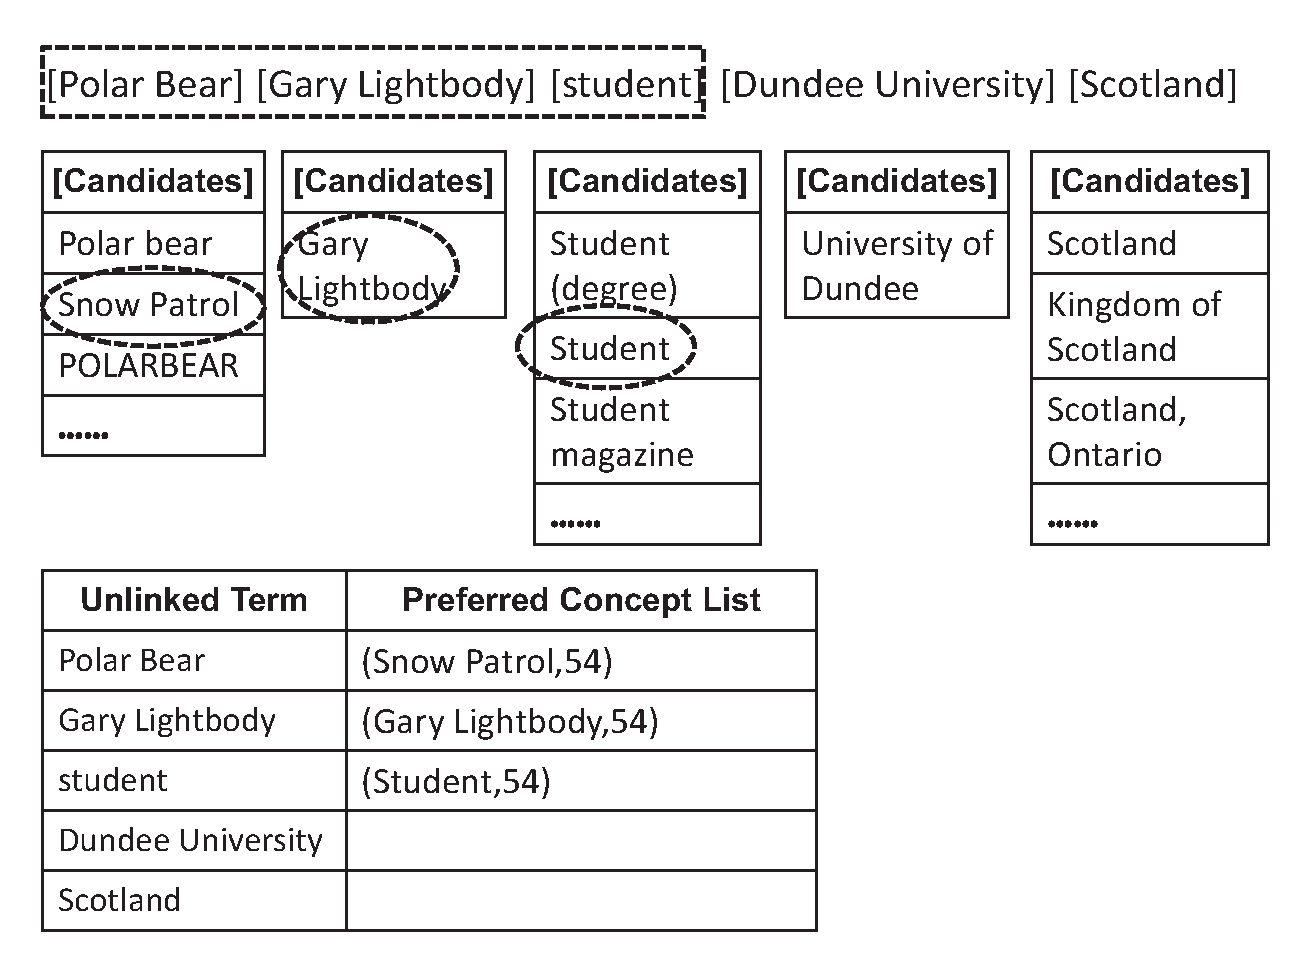
\epsfig{file=slidingwindow1.eps,width=1.2\columnwidth}
\caption{Step 1}
\label{fig:sw1}
\end{subfigure}
%\myskip
\begin{subfigure}[h]{0.8\columnwidth}
\centering
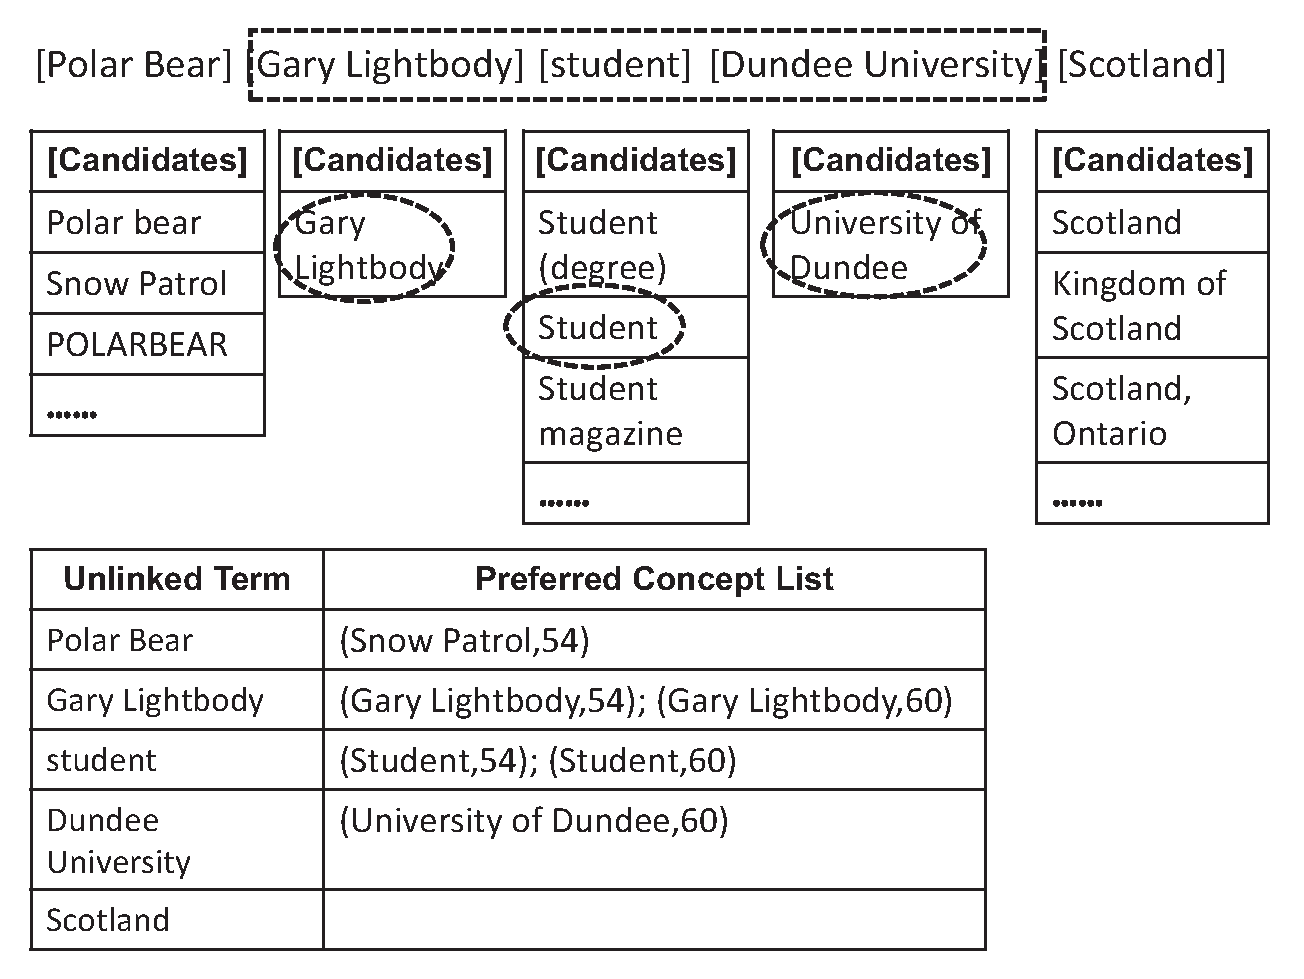
\epsfig{file=slidingwindow2.eps,width=1.2\columnwidth}
\caption{Step 2}
\label{fig:sw2}
\end{subfigure}
%\myskip
\begin{subfigure}[h]{0.8\columnwidth}
\centering
\epsfig{file=slidingwindow3.eps,width=1.2\columnwidth}
\caption{Step 3}
\label{fig:sw3}
\end{subfigure}
\caption{Sliding Window Example}
\label{fig:sw}
\end{figure}

\subsection{Wikify New Documents}
\label{sec:wikify}


%With the final co-occurrence matrix and appearance frequency of concepts generated after iteration,
%we can start our wikification process.
To wikify an entire document, our general idea is to
disambiguate several unlinked terms together within
a local context by optimizing the likelihood of co-occurrence among
a particular combination of senses for these terms. We could use
the whole document as the context but that will be computationally infeasible if
the document is large.
Instead we make the size of the context parameterized and tunable.
However, a local context can be misleading and can introduce errors in the
disambiguation. We solve this problem by creating a sliding window
that allows us to aggregate the disambiguation results from neighboring contexts
together and then make a pseudo-global decision about which sense each term
ultimately should have.

%What's
%different from the parsing result of Wikipedia corpus we use in the co-occurrence matrix enrichment
%phase is that this time we just have one kind of terms, which is unlinked term. All terms we
%recognize using our parser have a candidate Wikipedia concept list.
%All terms from the parse are unlinked terms.
%Unlike the enrichment phase, we have no linked term to help distinguish senses of the unlinked terms. So we come up with a method that uses the co-occurrence between candidate concepts to support
%one candidate concepts combination. To better explain our method, we first give some annotations here.

We illustrate this idea using \exref{ex-bear2} and show three steps
in sliding a window of size three in \figref{fig:sw}.
We parse the plain text using the NLP chunker discussed in Algorithm \ref{parsechunk}
and get the following terms: ``Polar Bear'', ``Gary Lightbody'', ``student'',
``Dundee University'' and ``Scotland''.
We create a candidate sense list for each term. Step 1 shows a window
containing ``Polar Bear'', ``Gary Lightbody'' and ``student''. Given that
each term has a few senses as candidates,
there are many combinations of senses for these three terms, such as:
\begin{itemize}
\item Polar bear, Gary Lightbody, Student (degree)
\shrink\item Snow Patrol, Gary Lightbody, Student
\shrink\item POLARBEAR, Gary Lightbody, Student (degree)
\end{itemize}
{\em Snow Patrol}, {\em Gary Lightbody} and {\em Student} turn out to be
the best sense combination since the sum of the {\em pair-wise}
co-occurrence is the largest at 54. Note here that we are simulating
the overall co-occurrence with pair-wise co-occurrence, which is a reasonable
approximation under computation constraints. We call the maximum sum
{\em sliding window score} ($S_{SW}$), and every term within this window
is associated with this disambiguation result (in the form of sense-$S_{SW}$ pair)
in a data structure called {\em Preferred Concept List} ($PCL$).

In Step 2, the window is slided to the right by one term, and the best
combination of senses is again computed while the $PCL$ is updated with three
more entries. This time $S_{SW}$ is 60.

In Step 3, within the last window of this sentence. The best combination
contains the {\em Student (degree)} sense, which is different from the result
of ``student'' in the 2 previous steps.

After we have finished sliding the window from start to finish, we group
the results for each term by senses and sum the $S_{SW}$ by the group.
In the case of ``student'', {\em Student} sense has a combined $S_{SW}$ of
114 while {\em Student (degree)} sense has a combined $S_{SW}$ of 25. The
first sense wins and becomes the final sense for the term ``student''.
Other terms are similarly disambiguated.

The detailed sliding window wikification algorithm is given in Algorithm
\ref{slide}. $L_u$ stands for the list of unlinked terms. $W_s$ stands for the
size of the sliding window. By picking one concept for each unlinked terms inside
the sliding window, we get a \emph{Concept Combination} ($CC$). 
Picking different candidate concepts from unlinked terms 
gives different $CC$s, thus forms the \emph{Concept Combination List} ($CCL$).
Therefore, $S_{SW}$ can be defined as
\[
S_{SW}=\max_{CC\in CCL}\sum_{c_i,c_j\in CC;i\neq j}{Co\left(c_i,c_j\right)}
\]
The $CC$ associated with $S_{SW}$ is called \emph{Best Concept Combination} ($BCC$).
$PCL_{L_u[i]}$ denotes the $PCL$ of the $i$th term in $L_u$.
%
%
%After parsing, we get a list of unlinked terms which represent the whole
%document, and it is denoted as $L_{T_u}$.
%We create a {\em sliding window} of $W_s$ consecutive terms. $W_s$ is the
%windows size which should not be confused with $W_c$ in \secref{sec:enrich}.
%The sliding window of terms basically create a segment of the article in which
%we try to disambiguate {\em all} the constituent terms together by maximizing a
%{\em sliding window score} (SWS). SWS is the sum of pair-wise concept
%co-occurrences.
%
%
%Each unlinked term $T_u$ in $L_{T_u}$ is associated
%with a data structure called \emph{Preferred Concept List}
%which is annotated as $PCL_{T_u}$. Each element in $PCL_{T_u}$ is a pair
%of a concept and a score known as {\em sliding window score} (SWS).
%
%When starting to wikify $T_u$ in $L_{T_u}$,
%we first pick the first $N$ terms from $L_{T_u}$.
%$N$ here is a parameter to set the size of the window containing all the currently handling terms. Not to confuse with the window
%we use in the matrix enrichment phase, we call this window \emph{Sliding Window}. By picking one
%candidate concept from each term in the sliding window, we get a combination of concepts with
%size $N$. We list all of the combinations of concepts in the sliding window.
%%We continue picking candidate concepts and finally get a list of combinations.
%The size
%of this list will be the product multiplied by the numbers of candidate concepts of all the terms in the
%sliding Window. We calculate a score for each combination by summing the co-occurrence frequency
%between each pair of candidate concepts. We sort the combination list by this score and pick up the
%rank 1 combination. In this combination, each term $T_u$ in the window has a chosen candidate concept.
%We then insert this chosen concept and the score of this combination to $PCL_{T_u}$.
%After updating of $PCL$, we slide the window one step forward to pick $N$ new terms and continue the process
%above, until we reach the end of $L_{T_u}$. Until now, each $T_u$ in $L_{T_u}$ has $PCL_{T_u}$ that
%may contain several elements. These elements are inserted when the sliding window move to
%different positions. Also, some elements may have the same concept. We scan the elements in $PCL_{T_u}$
%to calculate the score of each individual concept. The score of the same concept in different elements
%will be summed together. After that, we link $T_u$ to the concept with the highest score in $PCL_{T_u}$. However, if the highest score is 0, $T_u$ won't be assigned a link.
%When all the concepts of $T_u$ in $L_{T_u}$ are determined, the wikification process is done.

\begin{algorithm}[th]
\caption{Sliding Window Method}
\label{slide}
\begin{algorithmic}[1]
\Procedure{SlidingWindow}{$L_u$,$W_s$}
\For {$i \leftarrow 0,sizeof(L_u)-W_s$}
\State $CCL \leftarrow getCombination\left(L_u[i],W_s\right)$
\State Calculate $S_{SW}$ and $BCC$
%\State $BCC \leftarrow argmax_{CC\in CCL}\left(S_{SW}\left(CC\right)\right)$
\For {$j \leftarrow 0,sizeof(BCC)-1$}
\State Add $\langle BCC[j],S_{SW}\rangle$ to $PCL_{L_u[i+j]}$
\EndFor
\EndFor
\For {$i \leftarrow 0,sizeof(L_u)-1$}
\State Initialize $hash[concept \rightarrow score]$
\For {$j \leftarrow 0,sizeof(PCL_{L_u[i]})-1$}
\State $\langle key,value\rangle \leftarrow PCL_{L_u[i]}[j]$
%\If {$hash\;\;contain\;\;value$}
\State $hash[key] \leftarrow hash[key]+value$
%\Else
%\State $hash\left(key\right) \leftarrow value$
%\EndIf
\EndFor
\State $concept \leftarrow argmax_{key}\left(hash[key]\right)$
\If {$hash[concept]>0$}
\State Assign $concept$ to $L_u[i]$
\EndIf
\EndFor
\EndProcedure
\end{algorithmic}
\end{algorithm}

%\figref{fig:sw} shows a demonstration of the wikification process, taking the sentence we discuss in
%\secref{intro} as an example. After parsing, there are five unlinked terms recognized. Each unlinked term
%has a candidate concept list as is shown in \figref{fig:sw1}.
%The size of the sliding window is set to be 3. So in the first step of this process, the first
%three unlinked terms are taken into account.
%
%Then the $PCL$s of the first three terms are updated. ``Snow Patrol'' and the score 54 is inserted to the $PCL$
%of the first term. The updating of the other two terms are similar. After updating, we slide the window one step forward
%as is shown in \figref{fig:sw2}. This time, combination of ``Gary Lightbody'', ``Student'' and
%``University of Dundee'' is the best with score 60. Then the $PCL$s of the corresponding terms are updated.
%We continue slide the window until the last term is reached. After that, we scan the $PCL$ of each term to choose
%the best Wikipedia concept for it. Take ``Student'' as an example, the elements in its $PCL$ are:
%\begin{itemize}
%\item Student, 54
%\item Student, 60
%\item Student(degree), 25
%\end{itemize}
%The first two elements are of the same concept, so we sum the scores together. Then in ``Student'''s candidate
%concept list, ``Student'' has score 114, ``Student(degree)'' has score 25, others 0, so ``Student'' is chosen.
%
%Pseudo code is shown in Algorithm \ref{slide}.
%



